\documentclass[oneside, a4paper, 11pt]{article}

\usepackage{indentfirst}
\usepackage{listings}
\usepackage{graphicx}
\usepackage{float}
\usepackage{color}
\usepackage{amsmath}

\definecolor{codegreen}{rgb}{0,0.6,0}
\definecolor{codegray}{rgb}{0.5,0.5,0.5}
\definecolor{codepurple}{rgb}{0.58,0,0.82}
\definecolor{backcolour}{rgb}{0.95,0.95,0.92}
 
\lstdefinestyle{mystyle}{
    backgroundcolor=\color{backcolour},   
    commentstyle=\color{codegreen},
    keywordstyle=\color{magenta},
    numberstyle=\tiny\color{codegray},
    stringstyle=\color{codepurple},
    basicstyle=\footnotesize,
    breakatwhitespace=false,         
    breaklines=true,                 
    captionpos=b,                    
    keepspaces=true,                 
    numbers=left,                    
    numbersep=5pt,                  
    showspaces=false,                
    showstringspaces=false,
    showtabs=false,                  
    tabsize=2
}
 
\lstset{style=mystyle}

\begin{document}
\title{Java 8 Parallel Streams}
\author{Ethan Williams}
\date{\today}
\maketitle

\tableofcontents

% NOTES:
% Processing of parallel streams with JVM's ForkJoinPool.common() && calling thread
%  -Making own pool is an easy way to get around this
% Make mention of using thread-safe vs non thread-safe ds (probably in dangers section)

\setcounter{section}{-1}
\section{Prerequisites}
\subsection{Technical}
This document was written for Java developers who have an interest in using concurrency in streams, and as such assumes knowledge of serial streams and lambda expressions. Developers in other languages with similar mechanisms such as C\# with \verb|Linq| may also find the topics useful with the understanding that syntax, implementation, and functionality will differ.

Additionally, functional knowledge of \verb|java.util.concurrent| and the \verb|Consumer| interface will help in gaining a more practical knowledge but is not required.
\subsection{Language} \label{language}
Some of the language used in this paper may be ambiguous/confusing, the author's intended meanings for these terms are below:
\begin{itemize}
\item A stream instantiated with \verb|.stream()| only is referred to as a serial stream
\item A stream instantiated with \verb|.parallel().stream()| or \verb|.parallelStream()| is referred to as a parallel stream
\end{itemize}
\section{Introduction} % make content "basics" section of previous outline
Parallel streams were introduced into Java 8 alongside serial streams so that developers could utilize concurrency to make stream processing faster.  Concurrency allows the program to utilize threads, in the case of streams this is all handled by the JVM, in order to more efficiently utilize modern multiprocessor design.

Making a serial stream into a parallel stream is as easy as calling \verb|parallel()| after \verb|stream()|. In order for the \verb|parallel()| method to be applicable on the stream, the \verb|Collection| miust have an implementation of a \verb|Spliterator|, an object which can effectively break up a collection to be processed separately. 

Several operations are better suited to being used in parallel streams rather than serial streams, as is the case with \verb|Collector|s. Calling the \verb|collect()| method on the stream which will reduce and serialize it based on the behavior of the \verb|Collector| object passed as an argument. Parallel streams are better suited to using Collectors because reduction can only be accomplished this way whereas in serial streams there are several methods to accomplish this (although in many cases a \verb|Collector| is the best option).

Despite parallel streams being introduced into Java to simplify concurrency, developers can easily corrupt data and cause system bugs. This occurs due to developers not paying adequate attention to traditional Java concurrency practices as well as some of the special considerations with streams. %ADD CONTENT ABOUT SPECIFIC DANGERS
\section{Spliterator}
The \verb|Spliterator| is the backbone of parallel streams, allowing the program to split a collection apart and iterate through it. If a class extending a \verb|Collection| does not have a \verb|spliterator()| method returning a \verb|Spliterator| object, then Java is not able to process the collection with a parallel stream at all.

\subsection{Basics}
A Spliterator is an object which is represents the elements in a given range of the backing collection. At the beginning of a parallel stream there is one Spliterator that represents the entire collection. Calling the method \verb|trySplit()| will return a new Spliterator that represents the first half of untraversed elements while modifying the instance to represent the second half of untraversed elements. Figure \ref{fig:split} illustrates a call to \verb|trySplit()| on a Spliterator representing the entire collection.

\begin{figure}[H]
\centering
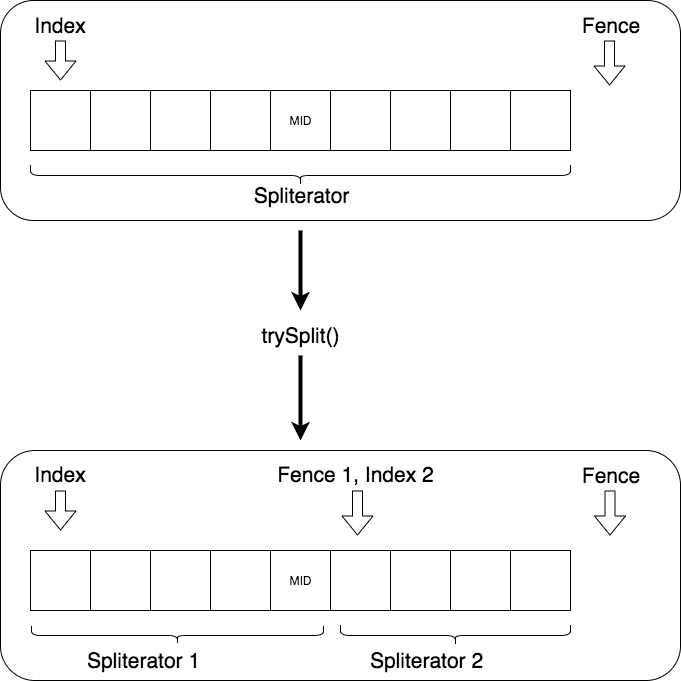
\includegraphics[width=8cm]{images/spliterator_illustrated.png}
\caption{A Spliterator before and after splitting}
\label{fig:split}
\end{figure}

\subsection{Implementation}
\textit{Spliterator implementations differ based on the collection so this section focuses on a simplified (easier to read) implementation of the Spliterator for Java's ArrayList.}

Spliterator has 3 instance fields: a backing collection, an index, and a fence. The backing collection for every Spliterator the entire collection it is based on. The index is the current cursor position of the Spliterator, which is analogous to the cursor position in an Iterator object. The fence is the index of the last element the Spliterator is responsible for plus one. The primary methods are \verb|tryEachRemaining()|, \verb|tryNext()|, \& \verb|trySplit()|. 

Although the cursor is similar to Iterator's, traversal through a Spliterator using \verb|tryEachRemaining()| and \verb|tryNext()| is different. \verb|tryEachRemaining()| in Figure \ref{fig:forEachRemaining} takes a Consumer object which is the operation to be executed on each element of the collection. A typical implementation will simply iterate through all elements and call the \verb|accept()| method on the consumer with the element as its only parameter. \verb|tryNext()| in Figure \ref{fig:tryAdvance} is similar although the operation is only attempted on element at the current cursor position. If that cursor position is past the fence of the Spliterator, then the method returns false, otherwise it returns true.

\begin{figure}[H]
\begin{lstlisting}[language=Java]
public void forEachRemaining(Consumer<? super E> action) {
    int i;
    if ((i = index) >= 0 && (index = fence) <= a.length) {
        for (; i < hi; ++i)  action.accept((E) list.elementData[i]);
    }
    throw new ConcurrentModificationException();
}
\end{lstlisting}
\caption{Implementation of forEachRemaining()}
\label{fig:forEachRemaining}
\end{figure}

\begin{figure}[H]
\begin{lstlisting}[language=Java]
public boolean tryAdvance(Consumer<? super E> action) {
    int hi = getFence(), i = index;
    if (i < hi) {
        index = i + 1;
        action.accept((E) list.elementData[i]);
        return true;
    }
    return false;
}
\end{lstlisting}
\caption{Implementation of tryAdvance()}
\label{fig:tryAdvance}
\end{figure}

Spliterator's primary functionality is encapsulated within the \verb|trySplit()| method in Figure \ref{fig:trySplit}. This implementation simply finds the midpoint and either returns a new \verb|Spliterator| from the cursor to the midpoint and the current instance of \verb|Spliterator| now covers mid to the fence. This is the code behind the split shown previously in FIgure \ref{fig:split}.

\begin{figure}[H]
\begin{lstlisting}[language=Java]
public Spliterator<E> trySplit() {
    int lo = index, mid = (lo + fence) >>> 1;
    return (lo >= mid) ? null : new Spliterator<E>(list, lo, index = mid);
}
\end{lstlisting}
\caption{Implementation of trySplit()}
\label{fig:trySplit}
\end{figure}

\section{Collectors}
A \verb|Collector| object defines a mutable reduction operation for a group of input elements, in other words a \verb|Collector| will put the elements of a stream into a container. The example shown in Figure \ref{fig:employee_collection} groups employees by department into a \verb|Map| object with the department as the key and a list of employees in that deparment as a value. \verb|Collector|s are commonly used for parallel operations as many data aggregations such as putting elements into a map are impossible to do without thread-safe data structures.

\begin{figure}[H]
\begin{lstlisting}[language=Java]
Map<Department, List<Employee>> byDept
    = employees.stream()
       .collect(Collectors.groupingBy(Employee::getDepartment));
\end{lstlisting}
\caption{Reduction of employees into map by a Collector}
\label{fig:employee_collection}
\end{figure}
\section{Practical Considerations when Using Parallel Streams}
Using parallel streams may seem easy but there are several common pitfalls for developers. These arise from not following good Java concurrency practices as well as an unawareness of how parallel streams are processed by the JVM.

One Java concurrency practice that is easy to forget using streams is the thread-safety of the data structures being used.

% see if I can get stats on simple degradation of performance using long-running op
Mistakes that can arise from not knowing Java's implementation can have arguably more severe consequences on application performance. One example relates to how the JVM breaks a parallel stream into threads. When a parallel stream is processes, the JVM begins by processing on the calling thread. As more subtasks are broken off, the JVM gets threads from \verb|ForkJoinPool.common()|, which is a common thread pool used in the background of the whole application. Since this is a common thread pool, one example of an error that could arise is if there is a long-running operation in a parallel stream. Each thread in the pool will be consumed executing that operation and subsequently all other JVM tasks using the common thread pool have to wait. This can lead to severe degradation in performance.
\end{document}